\documentclass[aspectratio=169]{beamer}

\usetheme{Boadilla}
\usefonttheme{professionalfonts}
\setbeamertemplate{navigation symbols}{}
\setbeamertemplate{itemize items}[circle]
\setbeamertemplate{enumerate items}[default]
\setbeamertemplate{headline}{}

\usepackage[utf8]{inputenc}
\usepackage[T1]{fontenc}
\usepackage{lmodern}
\usepackage{amsmath}
\usepackage{booktabs}
\usepackage{tabularx}
\usepackage{array}
\usepackage{hyperref}
\usepackage[strings]{underscore}
\usepackage{listings}
\usepackage{tikz}
\usetikzlibrary{arrows.meta,positioning,fit,calc,shapes.geometric}
\usepackage{xcolor}

\definecolor{courseblue}{HTML}{12355B}
\definecolor{coursegold}{HTML}{C98A2E}
\definecolor{courseice}{HTML}{EEF3F8}
\definecolor{coursegreen}{HTML}{2F6B4F}
\definecolor{coursegray}{HTML}{4B5563}
\definecolor{codebg}{HTML}{F7F9FC}
\definecolor{codecomment}{HTML}{5E6C84}
\definecolor{codestring}{HTML}{0B6E4F}

\setbeamercolor{palette primary}{bg=courseblue,fg=white}
\setbeamercolor{palette secondary}{bg=coursegold,fg=white}
\setbeamercolor{palette tertiary}{bg=courseblue,fg=white}
\setbeamercolor{palette quaternary}{bg=coursegold,fg=white}
\setbeamercolor{structure}{fg=courseblue}
\setbeamercolor{frametitle}{bg=courseice,fg=courseblue}
\setbeamercolor{title}{fg=courseblue}
\setbeamercolor{block title}{bg=courseblue,fg=white}
\setbeamercolor{block body}{bg=courseice,fg=black}
\setbeamercolor{normal text}{fg=black,bg=white}
\setbeamercolor{alerted text}{fg=coursegold}

\setbeamerfont{footline}{size=\scriptsize}

\setbeamertemplate{footline}{
  \leavevmode
  \hbox{
    \begin{beamercolorbox}[wd=.33\paperwidth,ht=2.8ex,dp=1.2ex,leftskip=0.8em]{palette primary}%
      University of Trieste
    \end{beamercolorbox}%
    \begin{beamercolorbox}[wd=.49\paperwidth,ht=2.8ex,dp=1.2ex,center]{palette tertiary}%
      \coursename{} \textbar{} \coursecode
    \end{beamercolorbox}%
    \begin{beamercolorbox}[wd=.18\paperwidth,ht=2.8ex,dp=1.2ex,rightskip=0.8em plus1fil]{palette secondary}%
      \insertframenumber{} / \inserttotalframenumber
    \end{beamercolorbox}%
  }
}

\hypersetup{
  colorlinks=true,
  linkcolor=courseblue,
  urlcolor=coursegreen
}

\lstdefinestyle{coursepython}{
  language=Python,
  basicstyle=\ttfamily\footnotesize,
  keywordstyle=\color{courseblue}\bfseries,
  commentstyle=\color{codecomment}\itshape,
  stringstyle=\color{codestring},
  showstringspaces=false,
  columns=fullflexible,
  keepspaces=true,
  frame=single,
  framerule=0.6pt,
  rulecolor=\color{courseblue},
  backgroundcolor=\color{codebg},
  xleftmargin=0.4em,
  xrightmargin=0.4em,
  aboveskip=0.4em,
  belowskip=0.2em
}

\newcommand{\coursename}{Data-driven Systems Engineering}
\newcommand{\coursecode}{440MI / 305SM}
\newcommand{\coursefooter}{}

\newcommand{\learninggoals}[1]{
  \begin{block}{Learning goals}
  #1
  \end{block}
}

\newcommand{\repoactivity}[1]{
  \begin{block}{Repo activity}
  #1
  \end{block}
}

\newcommand{\readinglist}[1]{
  \begin{block}{Papers and materials}
  {\footnotesize #1}
  \end{block}
}

\newcommand{\coursecontextframe}[5]{
  \begin{frame}{Course Map and Running Cases}
  \centering
  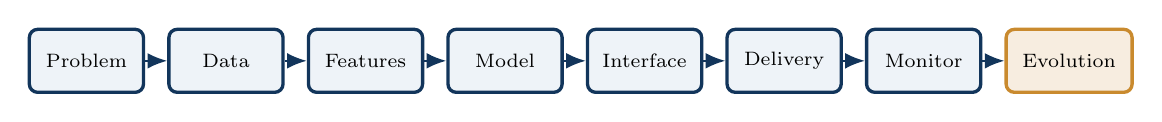
\begin{tikzpicture}[node distance=0.28cm]
  \node[flowbox, minimum width=1.45cm, minimum height=0.8cm] (problem) {\scriptsize Problem};
  \node[flowbox, minimum width=1.45cm, minimum height=0.8cm, right=of problem] (data) {\scriptsize Data};
  \node[flowbox, minimum width=1.45cm, minimum height=0.8cm, right=of data] (features) {\scriptsize Features};
  \node[flowbox, minimum width=1.45cm, minimum height=0.8cm, right=of features] (model) {\scriptsize Model};
  \node[flowbox, minimum width=1.45cm, minimum height=0.8cm, right=of model] (interface) {\scriptsize Interface};
  \node[flowbox, minimum width=1.45cm, minimum height=0.8cm, right=of interface] (delivery) {\scriptsize Delivery};
  \node[flowbox, minimum width=1.45cm, minimum height=0.8cm, right=of delivery] (monitor) {\scriptsize Monitor};
  \node[accentbox, minimum width=1.6cm, minimum height=0.8cm, right=of monitor] (evolution) {\scriptsize Evolution};
  \foreach \a/\b in {problem/data,data/features,features/model,model/interface,interface/delivery,delivery/monitor,monitor/evolution} {
    \draw[arrow] (\a) -- (\b);
  }
  \end{tikzpicture}

  \vspace{0.5em}
  \begin{block}{Today in the course}
  \textbf{Focus:} #1

  \textbf{Bridge:} #2
  \end{block}

  \begin{columns}[T]
  \column{0.48\textwidth}
  \begin{block}{Fraud case}
  {\footnotesize #3}
  \end{block}
  \column{0.48\textwidth}
  \begin{block}{Pasteurization case}
  {\footnotesize #4}
  \end{block}
  \end{columns}

  \vspace{0.3em}
  {\footnotesize \textbf{Course thread:} #5}
  \coursefooter
  \end{frame}
}

\newcommand{\classclosingframe}[4]{
  \begin{frame}{From This Class to the Next}
  \begin{block}{What stays with us}
  #1
  \end{block}

  \begin{columns}[T]
  \column{0.48\textwidth}
  \begin{block}{Project use}
  {\footnotesize #2}
  \end{block}
  \column{0.48\textwidth}
  \begin{block}{Next connection}
  {\footnotesize #3}
  \end{block}
  \end{columns}

  \vspace{0.3em}
  {\footnotesize \textbf{Course thread:} #4}
  \coursefooter
  \end{frame}
}

\tikzset{
  flowbox/.style={
    rounded corners=3pt,
    draw=courseblue,
    fill=courseice,
    very thick,
    minimum width=2.2cm,
    minimum height=0.9cm,
    align=center,
    font=\small
  },
  accentbox/.style={
    rounded corners=3pt,
    draw=coursegold,
    fill=coursegold!15,
    very thick,
    minimum width=2.2cm,
    minimum height=0.9cm,
    align=center,
    font=\small
  },
  arrow/.style={
    -{Latex[length=2.5mm,width=2mm]},
    thick,
    draw=courseblue
  }
}


\title{Class 2: Python, Data Quality, and Exploratory Analysis}
\author{\coursename}
\date{}

\begin{document}

\frame{\titlepage \coursefooter}

\begin{frame}{Agenda}
\begin{itemize}
\item Why Python is the working language of this course.
\item From business question to exploratory workflow.
\item Data quality dimensions and common failure modes.
\item EDA patterns for tabular, imbalanced, and streaming-flavored data.
\item How notebooks, pandas, and plotting libraries fit the engineering pipeline.
\end{itemize}
\coursefooter
\end{frame}

\begin{frame}{Learning goals}
\learninggoals{
\begin{itemize}
\item Explain why Python is effective for analysis, prototyping, and deployment.
\item Organize exploratory work into a reproducible ML workflow.
\item Evaluate data quality before talking about model quality.
\item Produce an EDA output that supports later feature engineering and modeling.
\end{itemize}
}
\coursefooter
\end{frame}

\coursecontextframe
{Data understanding and exploratory analysis.}
{This class moves from the business question into the data layer and prepares the observations we will later encode as features.}
{In the fraud case, EDA reveals imbalance, unusual value ranges, and the kinds of summaries needed before trustworthy modeling.}
{In the pasteurization case, EDA means inspecting sensor ranges, process states, and temporal patterns before building alerts or predictors.}
{The output of this class is not a model yet; it is a credible understanding of what the data can and cannot support.}

\begin{frame}{Why Python remains central}
\begin{itemize}
\item One language can cover data ingestion, analysis, modeling, APIs, dashboards, and automation.
\item The ecosystem is broad enough for both teaching and production-oriented prototypes.
\item The syntax is readable, which matters when notebooks become shared learning artifacts.
\item Python also integrates well with external services, files, and web frameworks.
\end{itemize}
\begin{block}{Important nuance}
Python is not always the fastest runtime, but it is often the fastest route from idea to tested workflow.
\end{block}
\coursefooter
\end{frame}

\begin{frame}{From problem statement to notebook workflow}
\begin{enumerate}
\item Define the decision or question.
\item Identify the dataset and its scope.
\item Check data quality and missingness.
\item Summarize distributions and relationships.
\item Form hypotheses for feature engineering and modeling.
\item Record risks, assumptions, and next steps.
\end{enumerate}
\repoactivity{
`notebooks/Class2_EDA.ipynb` and `Class2_EDA_Exercise.ipynb` already illustrate this transition from dataset inspection to structured analysis.
}
\coursefooter
\end{frame}

\begin{frame}[fragile]{Notebook step 1: load the Iris dataset}
\begin{lstlisting}[style=coursepython]
import pandas as pd
import seaborn as sns
import matplotlib.pyplot as plt

iris = sns.load_dataset("iris")
iris.head()
\end{lstlisting}
\begin{itemize}
\item The notebook begins with a compact import-and-load step so students can start exploration immediately.
\item Iris is intentionally simple: four numeric features and one class label.
\item This makes it easier to focus on process before complexity.
\end{itemize}
\coursefooter
\end{frame}

\begin{frame}[fragile]{Notebook step 2: inspect structure and missingness}
\begin{lstlisting}[style=coursepython]
iris.info()
iris.isnull().sum()
\end{lstlisting}
\begin{itemize}
\item `info()` summarizes schema, data types, and non-null counts.
\item `isnull().sum()` turns missingness into a concrete per-column check.
\item Even when the dataset is clean, this step trains a habit students will need later.
\end{itemize}
\coursefooter
\end{frame}

\begin{frame}{KDD and CRISP-DM in practical terms}
\begin{columns}[T]
\column{0.48\textwidth}
\textbf{KDD emphasis}
\begin{itemize}
\item Knowledge discovery
\item Data-driven pattern finding
\item Strong focus on analysis steps
\end{itemize}
\column{0.48\textwidth}
\textbf{CRISP-DM emphasis}
\begin{itemize}
\item Business understanding first
\item Structured iterative workflow
\item Better project communication
\end{itemize}
\end{columns}
\vspace{0.6em}
\begin{block}{Course perspective}
Students should know both, but CRISP-DM is usually easier to communicate in team projects because it begins from a decision need rather than a dataset alone.
\end{block}
\coursefooter
\end{frame}

\begin{frame}{Data quality is an engineering topic}
\begin{tabularx}{\textwidth}{>{\bfseries}l X}
Dimension & What to verify \\
\toprule
Accuracy & Are values plausible in the real domain? \\
Completeness & Are essential fields missing, null, or defaulted? \\
Consistency & Do categories, units, and timestamps match across sources? \\
Timeliness & Is the data still relevant for the decision we support? \\
Bias & Which users, behaviors, or operating states are underrepresented? \\
\bottomrule
\end{tabularx}
\coursefooter
\end{frame}

\begin{frame}{Better examples for EDA discussion}
\begin{itemize}
\item Fraud detection: class imbalance means plain accuracy can be dangerously misleading.
\item Titanic: missing values and categorical variables force explicit preprocessing choices.
\item Wine or Iris: useful for technique learning, but too clean to represent production reality.
\item Sensor streams: the same measurement may be normal in one operating state and abnormal in another.
\end{itemize}
\coursefooter
\end{frame}

\begin{frame}{What pandas contributes to the workflow}
\begin{itemize}
\item Loading and inspecting structured data quickly.
\item Profiling missing values, duplicates, and suspicious categories.
\item Reshaping, grouping, joining, and aggregating observations.
\item Time-aware analysis for event or sensor datasets.
\end{itemize}
\begin{block}{Why it matters}
If students cannot express data transformations clearly in pandas, they will struggle to make preprocessing reproducible later.
\end{block}
\coursefooter
\end{frame}

\begin{frame}{What plotting contributes}
\begin{tabularx}{\textwidth}{>{\bfseries}l X}
Matplotlib & Fine-grained control for reliable static plots and diagnostics. \\
seaborn & Faster statistical plots for distributions, pairwise relations, and summaries. \\
Notebook output & Good for exploratory storytelling, but should still be curated. \\
\end{tabularx}
\vspace{0.6em}
\begin{itemize}
\item Use plots to test hypotheses, not to decorate the notebook.
\item Every plot should answer a question: imbalance, drift hint, correlation, or anomaly.
\end{itemize}
\coursefooter
\end{frame}

\begin{frame}[fragile]{Notebook step 3: visualize distributions and relations}
\begin{lstlisting}[style=coursepython]
sns.pairplot(iris, hue="species", diag_kind="kde")
plt.show()

fig, axes = plt.subplots(2, 2, figsize=(12, 8))
sns.boxplot(x="species", y="sepal_length", data=iris, ax=axes[0, 0])
sns.boxplot(x="species", y="sepal_width",  data=iris, ax=axes[0, 1])
sns.boxplot(x="species", y="petal_length", data=iris, ax=axes[1, 0])
sns.boxplot(x="species", y="petal_width",  data=iris, ax=axes[1, 1])
\end{lstlisting}
\begin{itemize}
\item The pairplot gives a quick global view of separability and overlap.
\item The boxplots let students reason feature by feature instead of only visually scanning clusters.
\end{itemize}
\coursefooter
\end{frame}

\begin{frame}[fragile]{Notebook step 4: correlation and class distribution}
\begin{lstlisting}[style=coursepython]
plt.figure(figsize=(8, 6))
sns.heatmap(iris.drop("species", axis=1).corr(),
            annot=True, cmap="coolwarm")
plt.title("Correlation Matrix of Iris Features")
plt.show()

print(iris["species"].value_counts())
sns.countplot(x="species", data=iris, hue="species", palette="Set2")
\end{lstlisting}
\begin{itemize}
\item This matches the notebook's explicit check of both feature correlation and label balance.
\item It creates a natural comparison with future datasets where class balance is not this clean.
\end{itemize}
\coursefooter
\end{frame}

\begin{frame}[fragile]{Notebook step 5: grouped summaries and first hypotheses}
\begin{lstlisting}[style=coursepython]
iris.groupby("species").describe().T

iris.groupby("species").mean().plot(kind="bar", figsize=(10, 6))
plt.title("Mean Feature Values by Species")
plt.ylabel("Mean Value")
plt.show()
\end{lstlisting}
\begin{itemize}
\item Grouped descriptive statistics connect plotting with interpretation.
\item In the notebook, this is where students can argue that petal features separate species more clearly than sepal features.
\end{itemize}
\coursefooter
\end{frame}

\begin{frame}{What a good EDA output should contain}
\begin{itemize}
\item Descriptive summaries for numerical and categorical variables.
\item Missing-value patterns and candidate treatments.
\item Class balance or target behavior overview.
\item Correlation or dependency checks, including leakage suspicion.
\item A short list of modeling risks and feature ideas.
\end{itemize}
\coursefooter
\end{frame}

\begin{frame}{Common beginner mistakes}
\begin{itemize}
\item Starting model training before understanding the dataset.
\item Confusing a pretty chart with an informative chart.
\item Treating missing values as an inconvenience rather than a signal.
\item Ignoring the business meaning of columns because the code still runs.
\item Forgetting to document why a transformation was applied.
\end{itemize}
\coursefooter
\end{frame}

\begin{frame}{How the exercise notebook extends the workflow}
\begin{itemize}
\item `Class2_EDA_Exercise.ipynb` asks students to repeat the same sequence on Wine, Breast Cancer, and Digits.
\item This turns one notebook into a reusable method instead of a one-dataset example.
\item The key idea is transfer: the workflow stays stable even when the data semantics change.
\end{itemize}
\coursefooter
\end{frame}

\begin{frame}[fragile]{Exercise pattern for scikit-learn datasets}
\begin{lstlisting}[style=coursepython]
from sklearn.datasets import load_wine

wine = load_wine(as_frame=True)
df = wine.frame

df.head()
df.info()
df.isnull().sum()
df["target"].value_counts()
\end{lstlisting}
\begin{itemize}
\item This slide mirrors the exercise notebook and shows how the same EDA structure transfers to another source.
\item It also introduces the difference between a built-in seaborn dataset and a packaged scikit-learn dataset.
\end{itemize}
\coursefooter
\end{frame}

\begin{frame}{Technology links}
\readinglist{
\href{https://pandas.pydata.org/docs/}{pandas documentation};\ 
\href{https://matplotlib.org/stable/}{Matplotlib documentation};\ 
\href{https://jupyter.org/install}{Jupyter install guide};\ 
\href{https://scikit-learn.org/stable/}{scikit-learn documentation}.
}
\coursefooter
\end{frame}

\classclosingframe
{\begin{itemize}
\item EDA is not decoration; it is how we validate assumptions before modeling.
\item Python, pandas, and plots make data quality, target balance, and suspicious patterns visible.
\item Good exploration produces questions for preprocessing, feature design, and evaluation.
\end{itemize}}
{In the fraud and pasteurization cases, this is the stage where we inspect ranges, missingness, imbalance, time behavior, and candidate signals.}
{Class 3 uses that understanding to discuss PCA and dimensionality reduction when the feature space is large, redundant, or hard to visualize directly.}
{We first learn to see the data clearly, then we decide how to compress, transform, or model it.}

\begin{frame}{Papers and materials}
\readinglist{
\href{https://www.jmlr.org/papers/volume12/pedregosa11a/pedregosa11a.pdf}{Pedregosa et al. (2011), scikit-learn: Machine Learning in Python};\ 
\href{https://www.tandfonline.com/doi/abs/10.1080/01621459.1977.10480935}{Tukey (1977), Exploratory Data Analysis};\ 
\href{https://hdsr.mitpress.mit.edu/pub/9ymoz9h7}{Sambasivan et al. (2021), Everyone wants to do the model work, not the data work};\ 
\href{https://pandas.pydata.org/docs/getting_started/overview.html}{pandas overview}.
}
\coursefooter
\end{frame}

\end{document}
